\documentclass[11pt,a4paper]{article}
\usepackage[utf8]{inputenc}
\usepackage[vietnamese]{babel}
\usepackage{amsmath,amssymb}
\usepackage[version=4]{mhchem}
\usepackage{geometry}
\geometry{top=1.5cm,bottom=1.2cm,left=1.4cm,right=1.4cm,headheight=28pt,headsep=12pt,footskip=18pt}
\usepackage{graphicx}
\usepackage{xcolor}
\usepackage{tabularx}
\usepackage{array}
\usepackage{tikz}
\usepackage{fancyhdr}
\usepackage{enumitem}

\definecolor{hfRed}{HTML}{D32F2F}
\definecolor{hfGreen}{HTML}{8BC390}
\definecolor{mainGreen}{HTML}{2E7D32}
\definecolor{solBlue}{HTML}{1565C0}
\definecolor{tableGreen}{HTML}{E8F5E9}

\usepackage{ex_test}

\pagestyle{fancy}
\fancyhf{}
\renewcommand{\headrulewidth}{0.75pt}
\renewcommand{\headrule}{\hbox to\headwidth{\color{hfGreen}\leaders\hrule height \headrulewidth\hfill}}
\renewcommand{\footrulewidth}{0.75pt}
\renewcommand{\footrule}{\hbox to\headwidth{\color{hfGreen}\leaders\hrule height \footrulewidth\hfill}}

\fancyhead[L]{\small\itshape\color{hfRed}Tài liệu lưu hành nội bộ}
\fancyhead[R]{\small\color{hfRed}Thầy \textbf{TRẦN VĂN THẠNH} - 0777.470.803}

\fancyfoot[L]{\footnotesize\itshape\color{hfRed}CS1: 6/15 Nguyễn Hoàng, P. Kim Long, TP Huế \quad|\quad CS2: 24 Đặng Thái Thân, TP Huế}
\fancyfoot[R]{\small\textbf{\color{hfRed}Trang \thepage}}

\setlength{\parindent}{0pt}
\setlength{\parskip}{2pt}

\begin{document}

\begin{minipage}[t]{0.48\textwidth}
\textbf{TRƯỜNG ĐẠI HỌC KHOA HỌC}\\
\textbf{TRƯỜNG THPT CHUYÊN KHOA HỌC HUẾ}\\
\textit{ĐỀ CHÍNH THỨC}\\
\textit{(Đề thi có 04 trang)}
\end{minipage}
\hfill
\begin{minipage}[t]{0.48\textwidth}
\raggedleft
\textbf{\color{hfRed}ĐỀ KIỂM TRA GIỮA HỌC KỲ I -- NĂM HỌC 2026-2027}\\
\textbf{Môn: Hóa học -- Lớp 12 (CHUNG)}\\
\textit{Thời gian: 45 phút (không kể thời gian giao đề)}\\
\textbf{MÃ ĐỀ: 102}
\end{minipage}

\vspace{4pt}
\noindent
\textit{Họ và tên học sinh:} \dotfill \textit{Lớp:} \dotfill \textit{Số báo danh:} \dotfill

\vspace{3pt}
\noindent
\textit{\footnotesize (Cho nguyên tử khối: H = 1; C = 12; O = 16; Na = 23; Ag = 108)}

\vspace{3pt}
\hrule color{hfGreen} height 0.5pt


\vspace{4pt}
\noindent
{\color{mainGreen}\textbf{\Large A. TRẮC NGHIỆM (7,0 điểm)}}

\vspace{3pt}
\noindent
{\color{mainGreen}\textbf{\large PHẦN I (3,0 điểm). Câu trắc nghiệm nhiều phương án lựa chọn}}\\
\textit{\small Học sinh trả lời từ câu 1 đến câu 12. Mỗi câu hỏi chỉ chọn một phương án.}
\vspace{2pt}


\begin{ex}
Maltose là một loại disaccharide có nhiều trong mạch nha. Công thức phân tử của maltose là:
\choice
{\True $\ce{C12H22O11}$}
{$\ce{C6H12O6}$}
{$(\ce{C6H10O5})_n$}
{$\ce{C3H6O2}$}

\end{ex}

\begin{ex}
Tiến hành thí nghiệm glucose bị oxi hóa bởi thuốc thử Tollens theo các bước sau:\\
\textit{Bước 1:} Cho khoảng 2 mL dung dịch $\ce{AgNO3}$ 1\% vào ống nghiệm sạch.\\
\textit{Bước 2:} Thêm từ từ từng giọt dung dịch ammonia 5\%, lắc đều cho đến khi kết tủa tan hết. Dung dịch thu được là thuốc thử Tollens.\\
\textit{Bước 3:} Thêm tiếp khoảng 2 mL dung dịch glucose 2\% lắc đều. Sau đó, ngâm ống nghiệm vào cốc thuỷ tinh chứa nước nóng trong vài phút.\\
Phát biểu nào sau đây sai?
\choice
{Sản phẩm hữu cơ thu được sau bước 3 là ammonium gluconate}
{Sau bước 3, có lớp bạc (silver) kim loại bám trên thành ống nghiệm}
{\True Thí nghiệm trên chứng minh glucose có tính chất của polyalcohol}
{Trong phản ứng ở bước 3, glucose đóng vai trò là chất khử}

\end{ex}

\begin{ex}
Ethyl acetate được viết tắt là EtOAc, được sản xuất ở quy mô khá lớn để làm dung môi, là một loại hoá chất được sử dụng rất nhiều trong nước hoa, trong các loại sơn móng tay, hóa chất này rất phổ biến trong đời sống sinh hoạt hằng ngày. Ethyl acetate có công thức thu gọn nào sau đây?
\choice
{$\ce{CH3COOC6H5}$}
{\True $\ce{CH3COOC2H5}$}
{$\ce{CH3COOCH2CH2CH3}$}
{$\ce{CH3COOCH=CH2}$}

\end{ex}

\begin{ex}
Dầu mỡ để lâu bị ôi là do
\choice
{chất béo bị rữa ra}
{\True liên kết đôi C=C trong chất béo bị oxi hóa chậm bởi oxygen không khí tạo chất có mùi khó chịu}
{chất béo bị oxygen hoá chậm bởi oxygen không khí}
{chất béo bị thủy phân với nước trong không khí}

\end{ex}

\begin{ex}
Saccharose tham gia phản ứng nào sau đây?
\choice
{\True Phản ứng với $\ce{Cu(OH)2}$ tạo dung dịch màu xanh lam}
{Phản ứng với thuốc thử Tollens}
{Phản ứng với nước bromine}
{Phản ứng thuỷ phân trong môi trường kiềm}

\end{ex}

\begin{ex}
Thủy phân hoàn toàn 34,2 g saccharose trong môi trường acid. Khối lượng tổng glucose và fructose tạo thành (coi hiệu suất 100\%) là
\choice
{\True 36,0 g}
{18,0 g}
{34,2 g}
{68,4 g}

\end{ex}

\begin{ex}
Khi cho xà phòng vào nước cứng chứa ion $\ce{Ca^2+}$ và $\ce{Mg^2+}$, hiện tượng nào thường xảy ra?
\choice
{Nước cứng chuyển thành nước mềm ngay lập tức}
{\True Xà phòng tạo kết tủa với các ion $\ce{Ca^2+}$, $\ce{Mg^2+}$}
{Xà phòng bị oxi hóa thành chất béo}
{Xà phòng phân hủy hoàn toàn thành glycerol}

\end{ex}

\begin{ex}
Chất nào sau đây là chất béo bão hòa (ở trạng thái rắn ở nhiệt độ phòng)?
\choice
{Triolein}
{\True Tristearin}
{Trilinolein}
{Trioleate}

\end{ex}

\begin{ex}
Đun nóng 8,8 g ethyl acetate với 100 mL $\ce{NaOH}$ 1,00 M, phản ứng hoàn toàn. Khối lượng muối tạo thành là
\choice
{4,1 g}
{10,0 g}
{16,4 g}
{\True 8,2 g}

\end{ex}

\begin{ex}
Hợp chất nào sau đây được sử dụng làm chất giặt rửa tổng hợp?
\choice
{\True $\ce{CH3[CH2]11OSO3Na}$}
{$\ce{CH3COONa}$}
{$\ce{CH3[CH2]12COOCH3}$}
{$\ce{CH3[CH2]12COONa}$}

\end{ex}

\begin{ex}
Tinh thể chất rắn X không màu, vị ngọt, dễ tan trong nước. X có nhiều trong cây mía, củ cải đường và hoa thốt nốt. Trong công nghiệp, X được chuyển hóa thành chất Y dùng để tráng gương, tráng ruột phích. Tên gọi của X và Y lần lượt là
\choice
{\True Saccharose và glucose}
{Glucose và saccharose}
{Saccharose và cellulose}
{Glucose và fructose}

\end{ex}

\begin{ex}
Trong thí nghiệm điều chế ethyl acetate trong phòng thí nghiệm (cho ethanol, acetic acid và $\ce{H2SO4}$ đặc vào ống nghiệm rồi đun nhẹ), vai trò của $\ce{H2SO4}$ đặc là:
\choice
{\True chất xúc tác và hút nước để chuyển dịch cân bằng}
{chất môi trường kiềm để hòa tan ester}
{chất chỉ thị màu để nhận biết ester}
{chất oxi hóa alcohol thành aldehyde}

\end{ex}

\vspace{4pt}
\noindent
{\color{mainGreen}\textbf{\large PHẦN II (2,0 điểm). Câu trắc nghiệm đúng sai}}\\
\textit{\small Học sinh trả lời từ câu 1 đến câu 2. Trong mỗi ý a), b), c), d) ở mỗi câu, học sinh chọn Đúng hoặc Sai.}
\vspace{2pt}


\begin{ex}
Một ester no, đơn chức, mạch hở X có nguồn gốc từ quả táo tây có mùi thơm dễ chịu. Kết quả phân tích nguyên tố cho thấy X chứa 54,55\,\% carbon, 9,09\,\% hydrogen và 36,36\,\% oxygen về khối lượng. Từ phổ khối lượng (MS), xác định được tín hiệu ion phân tử $[\ce{M^+}]$ có $m/z = 88$. Cho 8,8 gam X tác dụng vừa đủ với 100 mL dung dịch $\ce{NaOH}$ 1 M, thu được muối Y và alcohol Z. Cho các nhận định sau:
\choiceTF
{\True Alcohol Z sinh ra là ethanol ($\ce{C2H5OH}$), có nhiệt độ sôi cao hơn ester X}
{Công thức phân tử của ester X là $\ce{C4H6O2}$}
{Tên gọi của X là methyl acetate}
{Đun nóng alcohol Z với $\ce{H2SO4}$ đặc ở $140^\circ\text{C}$ thu được alkene làm mất màu dung dịch nước bromine}

\end{ex}

\begin{ex}
Ngô và mía là hai nguyên liệu chính được sử dụng trong sản xuất ethanol. Tuy nhiên, chúng là những loại cây lương thực quan trọng. Trong khi đó, cellulose -- một nguồn nguyên liệu dồi dào và dễ tìm -- cũng có thể dùng để sản xuất ethanol. Tuy giá thành sản xuất ethanol từ cellulose còn cao, do quá trình nuôi cấy nấm sản sinh enzyme cellulase để thuỷ phân cellulose thành glucose tốn kém nhiều năng lượng, nhưng đây vẫn là một hướng đi đầy hứa hẹn trong tương lai.

\begin{center}
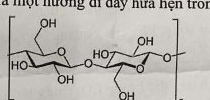
\includegraphics[width=6.5cm]{images_chuyen_khoa_hoc_hue_102/cellulose_clean.png}\\
\textit{\small Cấu trúc cellulose}
\end{center}

\choiceTF
{\True Phân tử cellulose được tạo thành từ nhiều đơn vị $\beta$-glucose, nối với nhau qua liên kết $\beta$-1,4-glycoside}
{Với những tiến bộ công nghệ đạt được, người ta tin rằng 0,81 tấn cellulose có thể sản xuất được 345 (L) ethanol. Khi đó, hiệu suất của quá trình đạt 70\,\% (cho biết khối lượng riêng của ethanol là 0,8 g/mL)}
{Cellulose có nhiều trong trái cây chín}
{\True Cellulose là một polymer mạch không phân nhánh}

\end{ex}

\vspace{4pt}
\noindent
{\color{mainGreen}\textbf{\large PHẦN III (2,0 điểm). Câu trắc nghiệm trả lời ngắn}}\\
\textit{\small Học sinh trả lời từ câu 1 đến câu 4. Viết đáp số tương ứng vào bài làm.}
\vspace{2pt}


\begin{ex}
Acid béo omega-3 và omega-6 là các acid béo không no với liên kết đôi đầu tiên ở vị trí số 3 và 6 khi đánh số từ nhóm methyl. Acid béo omega-3 và omega-6 đều có vai trò quan trọng đối với cơ thể, giúp phòng ngừa nhiều loại bệnh. Linoleic acid có công thức cấu tạo như sau:

\begin{center}
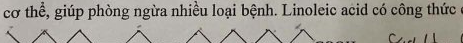
\includegraphics[width=9.0cm]{images_chuyen_khoa_hoc_hue_102/linoleic_clean.png}
\end{center}

Linoleic acid thuộc loại acid béo omega-x và có phân tử khối là y. Số có giá trị 10y+x là bao nhiêu?


\noindent\textit{Trả lời:} \dotfill

\end{ex}

\begin{ex}
Methyl salicylate dùng làm thuốc xoa bóp giảm đau, được điều chế theo phản ứng sau:
$$\ce{HOC6H4COOH + CH3OH <=>[\ce{H2SO4}, t^o] HOC6H4COOCH3 + H2O}$$

\begin{center}
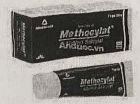
\includegraphics[width=4.5cm]{images_chuyen_khoa_hoc_hue_102/methocylat.png}
\end{center}

Để sản xuất 3,8 triệu tuýp thuốc xoa bóp giảm đau cần tối thiểu m tấn axit salixylic. Biết mỗi tuýp thuốc chứa 2,8 gam methyl salicylate và hiệu suất phản ứng tính theo axit salixylic là 80\,\%. Tính giá trị của m ? (Kết quả làm tròn đến con số thứ nhất sau dấu phẩy).


\noindent\textit{Trả lời:} \dotfill

\end{ex}

\begin{ex}
Đun nóng một loại mỡ động vật với dung dịch $\ce{KOH}$, sản phẩm thu được có chứa muối potassium stearate ($\ce{C17H35COOK}$). Phân tử khối của potassium stearate là bao nhiêu ?


\noindent\textit{Trả lời:} \dotfill

\end{ex}

\begin{ex}
Một xưởng sản xuất gương phẳng cần tráng bạc lên $15\,000\text{ m}^2$ bề mặt kính. Biết khối lượng bạc cần phủ trên mỗi mét vuông bề mặt kính là 0,8 gam. Lớp bạc được tạo thành bằng phản ứng tráng bạc của glucose với thuốc thử Tollens (được điều chế từ dung dịch $\ce{AgNO3}$ và $\ce{NH3}$). Giả sử $\ce{AgNO3}$ được sử dụng dư và hiệu suất tạo bạc bám trên bề mặt kính tính theo glucose đạt 80\,\%. Tính khối lượng glucose tối thiểu (theo kg) cần dùng để sản xuất số gương trên (làm tròn đến hàng đơn vị).


\noindent\textit{Trả lời:} \dotfill

\end{ex}

\vspace{6pt}
\noindent
{\color{mainGreen}\textbf{\Large B. TỰ LUẬN (3,0 điểm)}}
\vspace{2pt}


\begin{ex}
\textbf{(1,0 điểm)} Cây xanh nhả khí oxygen sau khi hoàn tất quá trình quang hợp, con người và nhiều loài động vật khác cần khí oxygen để duy trì sự sống. Phản ứng quang hợp được mô tả theo phương trình sau:
$$n\,\ce{CO2} + m\,\ce{H2O} \xrightarrow{\text{ánh sáng / chất diệp lục}} \ce{C_n(H2O)_m} + n\,\ce{O2}$$
Giả sử một cây xanh trưởng thành tiêu thụ lượng $\ce{CO2}$ trung bình khoảng 22 kg/năm để thực hiện quá trình quang hợp và trung bình một năm mỗi người cần tối thiểu 1,2 tấn oxygen để duy trì sự sống. Để cung cấp đủ lượng oxygen cho 7,8 tỉ người trên Trái đất trong một năm thì cần bao nhiêu tỉ cây xanh như trên?


\vspace{4.0cm}

\end{ex}

\begin{ex}
\textbf{(1,0 điểm)} Viết công thức cấu tạo và gọi tên các đồng phân ester có công thức phân tử $\ce{C4H8O2}$.


\vspace{3.5cm}

\end{ex}

\begin{ex}
\textbf{(1,0 điểm)} Một nhà máy đường sản xuất saccharose tinh khiết từ cây mía tươi. Biết rằng trong mía tươi chứa 13,5\,\% saccharose về khối lượng và hiệu suất thu hồi saccharose của toàn bộ quy trình sản xuất đạt 82\,\%. Tính khối lượng mía tươi (theo tấn) tối thiểu cần cung cấp cho nhà máy để sản xuất được 1,0 tấn đường saccharose tinh khiết (làm tròn đến hàng phần trăm).


\vspace{3.5cm}

\end{ex}

\vspace{8pt}
\begin{center}
\textbf{-------------------- HẾT --------------------}\\
\textit{\small (Học sinh không được sử dụng tài liệu -- Giám thị không giải thích gì thêm)}
\end{center}

\end{document}
